% Section 09: Conclusion
% Mode: Mixed — summarize contributions (descriptive), acknowledge limitations
%   (interpretive), future research (forward-looking)

\section{Conclusion}\label{sec:conclusion}

\subsection*{Introduction}

This section draws conclusions from the findings, identifies contributions to
practice, and acknowledges limitations. Theoretical contributions and future
research directions are presented in the \textit{Discussion} (Section~\ref{sec:discussion}). The
following subsections detail these conclusions:

\localtableofcontents\clearpage

%% ================================================================
%% 7.1 Research Questions Revisited
%% ================================================================
\subsection{Research Questions Revisited}\label{subsec:rqs-revisited}

The central research question asked: \textit{What practices do Enterprise
Architecture (EA) practitioners adopt when using Generative AI (GenAI) for
Reference Architecture (RA) development, and how can these be systematized into
guidance?} The Design-Oriented Delphi methodology, conducted across three
rounds with eight to ten participants, produced convergent answers through four
sub-questions.

\textbf{sRQ1: What GenAI practices are EA practitioners currently using?}
The Delphi panel identified and validated seven practice categories:
System/Codebase Analysis, Research \& Exploration, Adversarial Review,
Governance/Compliance Checking, First Draft \& Documentation, Stakeholder
Communication, and Deep Workflow Integration (Section~\ref{subsec:srq1}).
\textit{Conclusion:} EA practitioners have developed structured,
category-specific GenAI practices within months of tool availability. The strong consensus on System/Codebase Analysis and the weaker consensus on
Stakeholder Communication suggest that GenAI adds more value where less
organizational context is needed.

\textbf{sRQ2: What changes to EA practice are practitioners experiencing?}
Three interrelated shifts emerged: the verification burden shift, the
creator-to-curator transformation, and changing cross-role dynamics
(Section~\ref{subsec:srq2}). \textit{Conclusion:} GenAI integration
restructures the practitioner's role from content creator to content curator.
The verification burden shift is the most significant change, indicating that
quality assurance, not content generation, is the primary challenge.

\textbf{sRQ3: How do practitioners make sense of impacts and trade-offs?}
The panel articulated eight verification heuristics in two tiers, anchored by
trust calibration and the junior colleague mental model
(Section~\ref{subsec:srq3}). \textit{Conclusion:} Practitioners navigate
GenAI integration through calibrated trust rather than binary accept/reject
decisions. The junior colleague metaphor provides a shared cognitive frame
for positioning GenAI contributions within the team.

\textbf{sRQ4: How should practices be systematized into guidance?}
The guidance artifact (Section~\ref{sec:artifact}) organizes recommendations
at three levels: directive, contextual, and adaptive
(Section~\ref{subsec:srq4}). \textit{Conclusion:} Effective guidance must
respect the variability in practitioner consensus. A single set of
prescriptive rules would not serve a phenomenon where GenAI value ranges from
consistently high (codebase analysis) to heavily context-dependent
(stakeholder communication).

Table~\ref{tab:conclusion-summary} summarizes these conclusions.
Figure~\ref{fig:conclusions-framework} maps them back onto the conceptual
framework introduced in Section~\ref{sec:conceptualframework}, showing how each
sub-question produced a distinct finding within the practice evolution cycle.

\begin{table}[ht]
    \centering
    \caption{Summary of Research Question Conclusions}
    \label{tab:conclusion-summary}
    \begin{tabular}{|p{1.8cm}|p{4.5cm}|p{7.5cm}|}
        \hline
        \textbf{Sub-RQ} & \textbf{Question Focus} & \textbf{Conclusion} \\
        \hline
        sRQ1 & Current GenAI practices & Seven validated practice categories spanning RA development, from System/Codebase Analysis (strongest consensus) to Deep Workflow Integration (emerging). \\
        \hline
        sRQ2 & Changes to EA practice & Three practice evolution shifts: verification burden shift, creator-to-curator transformation, and changing cross-role dynamics. \\
        \hline
        sRQ3 & Sense-making of impacts & Eight verification heuristics in two tiers (structural and domain), anchored by trust calibration and the junior colleague mental model. \\
        \hline
        sRQ4 & Systematization into guidance & Three-tiered guidance artifact: directive (high consensus), contextual (moderate), and adaptive (high variability), organized by practice category. \\
        \hline
    \end{tabular}
\end{table}

\begin{figure}[ht]
    \centering
    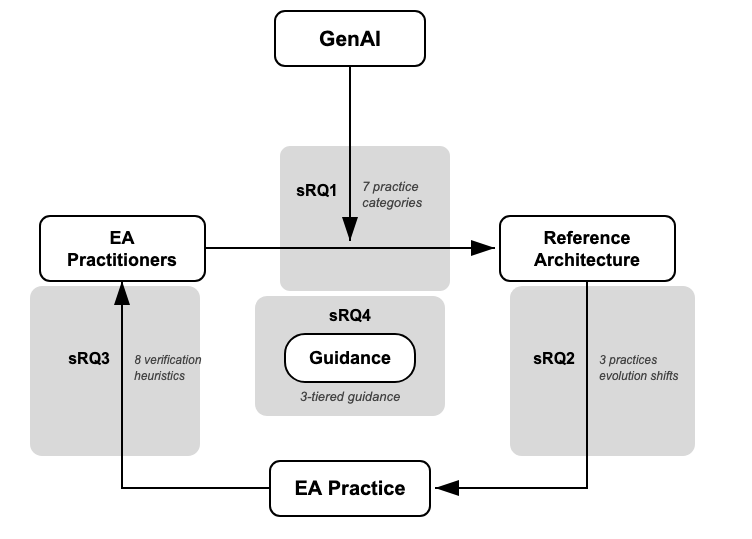
\includegraphics[width=0.75\textwidth]{images/conceptual_model_conclusion.png}
    \caption[Research conclusions mapped to the analytical framework.]{Research conclusions mapped to the analytical framework (cf. Figure~\ref{fig:analytical-framework}).}
    \label{fig:conclusions-framework}
\end{figure}

\textbf{Overall conclusion:} EA practitioners are developing structured,
category-specific practices for GenAI integration, and these practices can be
systematized through consensus-validated guidance that respects the variability
inherent in context-dependent architectural work.

%% ================================================================
%% 7.2 Contributions
%% ================================================================
\subsection{Contributions}\label{subsec:contributions}

Theoretical contributions (extending distributed cognition, practice theory,
and the junior colleague mental model as calibration heuristic) are developed
in Section~\ref{subsec:disc-implications-theory}. Here we summarize the
practical contributions.

\subsubsection{Contributions to Practice}

Five practical contributions emerge from these results. First, the practice
taxonomy describes what practitioners actually do with GenAI, not what the
technology can theoretically do. Each of the seven categories maps to specific
RA development activities and gives organizations a shared vocabulary for
discussing GenAI integration.

Second, the consensus--variability profiles reveal where GenAI adds consistent
value and where its contribution remains contested. System/Codebase Analysis
($M = 4.00$, $SD = 0.82$) represents a zone of reliable augmentation, while
Stakeholder Communication ($M = 3.00$, $SD = 1.37$) marks the organizational
context boundary where GenAI value depends heavily on local conditions.

Third, the guidance artifact offers graduated entry points with embedded
traceability mechanisms (verification heuristics, stakeholder-fit checks, and
trust calibration references) at each practice level. Practitioners new to
GenAI integration can begin with directive-level practices where consensus is
strong, then progress to adaptive practices as they develop calibration skills.
This structure addresses the guidance vacuum identified in
the \textit{Introduction} (Section~\ref{sec:introduction}): the absence of evidence-based
understanding, evaluation frameworks, risk management guidance, and shared
vocabulary for GenAI-augmented EA practice.

Fourth, the gate-to-guardrail governance transition addresses a practical
problem: when anyone with GenAI can produce architectural artifacts, periodic
review boards cannot keep up. Encoding architectural constraints as
machine-readable rules and checking them continuously gives organizations a
governance pathway that scales with GenAI-accelerated artifact production.

Fifth, the anti-atrophy strategies address a concrete risk: practitioners lose
skills they stop exercising, and GenAI automates precisely the skills (cold-start
writing, exhaustive research, cover-to-cover reading) through which architectural
expertise develops \parencite{kabashkin_cognitive_atrophy_2025}. Three friction
strategies (AI-free design sessions, attempt independently first, pair
programming mindset) help practitioners maintain the independent capability that
makes trust calibration possible.

%% ================================================================
%% 9.3 Limitations
%% ================================================================
\subsection{Limitations}\label{subsec:concl-limitations}

\textit{Limitations} (Section~\ref{subsec:disc-limitations}) detailed six categories of limitations
qualifying these findings. Three merit brief restatement here so the conclusion
stands independently. First, the Delphi panel comprised eight to ten
participants drawn from the researcher's professional network, limiting generalizability and introducing self-selection bias toward early
adopters. Second, all findings represent a temporal snapshot from January to
March 2026; GenAI capabilities evolve rapidly, and specific tool-dependent
practices may shift within months. Third, practice data is self-reported through
workbooks and facilitated sessions rather than directly observed, introducing
potential recall and social desirability biases. One additional qualification
bears emphasis: these are early-adopter findings, producing a portrait of
frontier practice that may not generalize to the broader EA practitioner
population as adoption matures.

